\documentclass[12pt,a4paper]{article}

% Required packages
\usepackage[utf8]{inputenc}
\usepackage[T1]{fontenc}
\usepackage{graphicx}
\usepackage{geometry}
\usepackage{wrapfig}
\usepackage{listings}
\usepackage{xcolor}
\usepackage{hyperref}
\usepackage{pgfplots}
\pgfplotsset{compat=1.18}
\usepackage{float}
\usepackage{amsmath}
% Allow more floats at the top of the page (figures)
\renewcommand{\topfraction}{0.95}
\renewcommand{\floatpagefraction}{0.9}
\renewcommand{\textfraction}{0.05}
\setcounter{topnumber}{5}
\setcounter{totalnumber}{10}

\definecolor{codegreen}{rgb}{0,0.6,0}
\definecolor{codegray}{rgb}{0.5,0.5,0.5}
\definecolor{codepurple}{rgb}{0.58,0,0.82}
\definecolor{backcolour}{rgb}{0.95,0.95,0.92}

\lstdefinestyle{codeListingStyle}{
    backgroundcolor=\color{backcolour},   
    commentstyle=\color{codegreen},
    keywordstyle=\color{magenta},
    numberstyle=\tiny\color{codegray},
    stringstyle=\color{codepurple},
    basicstyle=\ttfamily\footnotesize,
    breakatwhitespace=false,         
    breaklines=true,                 
    captionpos=b,                    
    keepspaces=true,                 
    numbers=left,                    
    numbersep=5pt,                  
    showspaces=false,                
    showstringspaces=false,
    showtabs=false,                  
    tabsize=2
}

% Set page margins
\geometry{top=0cm, bottom=2cm, left=2cm, right=2cm}

\begin{document}

% Remove page numbers
\pagestyle{empty}

% Add image at the top of the page
\begin{figure}[t!]
    \centering
    \includegraphics[width=1\textwidth]{images/PJATK_PL_poziom_1.png}
    \label{fig:top-image}
\end{figure}

% Centered content
\begin{center}
\vspace{2cm}

{\Large \textbf{Wydział Informatyki}}

\vspace{1.5cm}

{\large  \textbf{Systemy Inteligentne i Data Science}}

\vspace{0.5cm}

Inteligentne Systemy Przetwarzania Danych

\vspace{2cm}

{\large  \textbf{Michał Lichtarski}} \\
Nr albumu s27643

\vspace{1cm}

{\large  \textbf{Marcin Ziółkowski}} \\
Nr albumu s27597

\vspace{2cm}

{\Large \textbf{Tytuł pracy dyplomowej}}

\end{center}

\vfill

\begin{flushleft}
\hspace*{0.5\textwidth}Praca inżynierska \\
\hspace*{0.5\textwidth}Promotor Adam Szmigielski
\end{flushleft}

\vspace{2.5cm}

\begin{center}
Warszawa, luty, 2025
\end{center}

\newgeometry{top=2cm, bottom=2cm, left=2cm, right=2cm}
\section*{Streszczenie}

Celem niniejszej pracy jest przedstawienie działania oraz implementacji równoległego silnika szachowego opartego na algorytmie przeszukiwania drzewa Monte Carlo wspomaganego siecią neuronową. Zostanie przedstawiony proces przetwarzania danych szachowych wraz z niezbędną modyfikacją biblioteki szachowej.
W pracy zostaną omówione ulepszenia zarówno sieci neuronowej jak i samego MCTS, które zostały wprowadzane na przestrzeni ostatnich kilku lat. Na końcu zostaną przedstawione wyniki ewaluacji samej sieci neuronowej oraz porównanie opisywanego silnika z silnikiem Stockfish.

\textbf{Słowa kluczowe} – monte carlo tree search, sieć neuronowa, szachy, wieloprocesowość

\section*{Wstęp}

Żyjemy w dynamicznie rozwijającym się technologicznie świecie, w którym algorytmy uczenia maszynowego odgrywają coraz to większą rolę w różnych dziedzinach życia. Możemy je spotkać nawet w szachach. Prawie każdy z nas zna strony internetowe gdzie można rywalizować z różnymi graczami, czy nawet z modelami. Dla zobrazowania jak algorytmy szachowe są skomplikowanym zadaniem Claude Shannon w swoim artykule z 1950 roku \textit{Programming a Computer for Playing Chess} oszacował, że liczba wszystkich różnych kombinacji partii w szachach wynosi około $10^{120}$, co jest nazwane dzisiaj liczbą Shannon'a. Również opisał jak powinien wyglądać algorytm heurystyczny, który bierze pod uwagę najbardziej obiecujące ruchy "Select the variations to be explored by some process so that the machine does not waste its time in totally pointless variations.". Gdyż jak sam podkreślił, metodą brute force jest to nieosiągalne. Dało to początek rozwoju algorytmów takich jak minimax, czy monte Carlo tree search, które są obecnie szeroko stosowane do dzisiaj.

Jak bardzo zmieniły się algorytmy szachowe na przestrzeni lat dobrze obrazuje książka Huberta Dreyfusa \textit{Alchemy and Artificial Intelligence} z 1965 roku, w której autor napisał że nie ma obecnie algorytmu szachowego, który byłby wstanie grać na amatorskim poziomie "Still no chess program can play even amateur chess". Gdzie zaledwie 20 lat później, w 1988 roku, program szachowy \textit{Deep Thought} wygrał z arcymistrzem szachowym Bentem Larsenem. W 1997 roku komputer \textit{Deep Blue} pokonał Kasparowa w meczu z standardową kontrolą czasu, a w 2017 roku program AlphaZero opracowany przez Google pokonał algorytmy szachowe, takie jak Stockfish i Elmo.
\section*{Format danych PGN}
Fromat PGN jest powszechnie stosowanym sposobem pechowywania partii szachowych. W danym pliku może znajdować się dowolna ilość gier. Każda z nich ma między innymi nazwy graczy, wynik oraz stos ruchów. Taki sposób zapisu jest bardzo efektywny pamięciowo, gdyż nie zapisuje on pozycji na planszy w każdej turze, a jedynie wykonywane ruchy. Dodatkowym atutem jest gotowa biblioteka python-chess\footnote{https://python-chess.readthedocs.io/} do dekodowania pliku oraz rozgrywania partii.

\vspace{0.5cm}

\begin{lstlisting}[
    language=Python, 
    caption=przykład pliku PGN,
    inputencoding=utf8,
    basicstyle=\ttfamily\footnotesize,
    xleftmargin=0.1cm,
    showspaces=false,
    showstringspaces=false,
    showtabs=false,
    keepspaces=true
]
[Event "F/S Return Match"] 
[Site "Belgrade, Serbia JUG"] 
[Date "1992.11.04"] 
[Round "29"] 
[White "Fischer, Robert J."]
[Black "Spassky, Boris V."] 
[Result "1/2-1/2"] 

1. e4 e5 2. Nf3 Nc6 3. Bb5 a6 4. Ba4 Nf6 5. O-O Be7 6. Re1 b5 7. Bb3 d6 ...
\end{lstlisting}
\section*{Przetwarzanie danych}
Dane użyte do wstępnego trenowania modelu zostały pobrane ze strony pgnmentor\footnote{https://www.pgnmentor.com/}. Przy ich pobieraniu brany był uwagę ranking graczy. Dane z zawodów nie były używane ze zwględu na różne niestandardowe układy figur na planszy, co wprowadzało błędy. Do przetworzenia danych została stworzona klasa PGNDataset. Jej zadaniem jest utworzenie plików o rozszerzeniu .rdg, które zawierają zserializowany obiekt krotki. Rozbicie danych gier na kilka plików zostało podyktowane ograniczeniami pamięci dynamicznej procesora oraz procesora graficznego. Każdy z nich zawiera z góry ustaloną ilość zakodowanych partii, dzięki czemu w prosty sposób można zarządzać wielkością pliku, a tym samym ilością zajętej pamięci graficznej, co ma bardzo duży wpływ na prędkość trenowania modelu. W przypadku za dużego pliku karta graficzna musi używać współdzielonej pamięci, co znacznie spowalnia proces trenowania ze względu na konieczność przesyłania danych pomiędzy pamięcią ram, a vram. W przypadku zbyt małych plików, podczas procesu trenowania trzeba często wczytywać dane z dysku do ramu \footnote{Systemy operacyjne są w stanie cache'ować często używane dane w pamięci dynamicznej. W dystrybucji Ubuntu można zauważyć w system monitorze pod nazwą "Cache"}, a następnie przesyłać je do karty, co również spowalnia cały proces.

\section*{Klasa PGNDataset}
Działanie klasy rozpoczyna się od metody \textit{encode directory}, która przyjmuje ścieżke do katalogu z plikami \textit{.pgn}. Następnie iteruje po wszystkich plikach. Dla każdej gry z pliku wywołuje metodę \textit{encode game}, której listing jest przedstawiony pod spodem. Enkoduje ona ruchy, plansze oraz wynik partii i zwraca je w postaci trzech tablic numpy. Po przetworzeniu odpowiedniej ilości gier, są one zapisywane do pliku \textit{.rdg} w postaci krotki. Dodatkowo ze względu na model, który uczy się jedynie ruchów dla białych figur, obracana jest plansza po przekątnej. Dzięki temu zmieniamy perspektywę gracza. Działa to identycznie tak jakbyśmy w rzeczywistości zamienili się miejscem z przeciwnikiem. W przypadku zmiany perspektywy planszy, również jest zmieniana perspektywa ruchu oraz odwracany jest wynik partii. 

\lstset{style=codeListingStyle}
\begin{lstlisting}[
    language=Python, 
    caption=Metoda encode game,
    inputencoding=utf8
]
def encode_game(self, game: chess.pgn.Game):
        board = BoardPlus()
        moves, boards, wins = [], [], []

        for move in game.mainline_moves():
            real_board.push(move)
            if board.changed_perspective:
                move = BoardPlus.change_move_perspective(move)

            moves.append(board.encode_move(move))
            boards.append(board.encode())
            wins.append(self.white_win(game) * (1 if not board.changed_perspective else -1))
            board.better_push(move)

            board.change_perspective()
        return np.array(moves), np.array(boards), np.array(wins)
\end{lstlisting}

\section*{Przechowywanie zakodowanych gier w pamięci programu}
Dane w postaci list zwracane przez metodę \textit{encode game} są dodawane do kolejnych trzech list \textit{games move}, \textit{games board} oraz \textit{games win}. Po przetworzeniu odpowiedniej ilości gier są one scalane za pomocą metody \textit{concatenate} i zapisywane do pliku. Taki nietypowy sposób przechowywania został zastosowany ze względów wydajnościowych. Przy użyciu jednowymiarowych list, po każdym wywołaniu metody \textit{enocde game}, trzeba by używać \textit{concatenate} do scalania danych, co jest bardzo nieefektywne. Wraz z wielkością list, czas wykonania rośnie znacząco co można zaobserwować na poniższym wykresie.

\lstset{style=codeListingStyle}
\begin{lstlisting}[
    language=Python, 
    caption=Fragment metody encode directory,
    inputencoding=utf8
]
game_moves, game_boards, game_wins = self.encode_game(game)

if len(game_moves) == 0 or len(game_boards) == 0 or len(game_wins) == 0:
    continue
games_move.append(game_moves)
games_board.append(game_boards)
games_win.append(game_wins)

PGNDataset.number_converted_games += 1
if PGNDataset.number_converted_games % max_games_in_file == 0:
    moves, boards, wins = np.concatenate(games_move), np.concatenate(games_board), np.concatenate(games_win)
    PGNDataset.save_games_data_to_file((moves, boards, wins), output_path)
    games_move, games_board, games_win = [], [], []
\end{lstlisting}

\begin{figure}[!t]
    \centering
    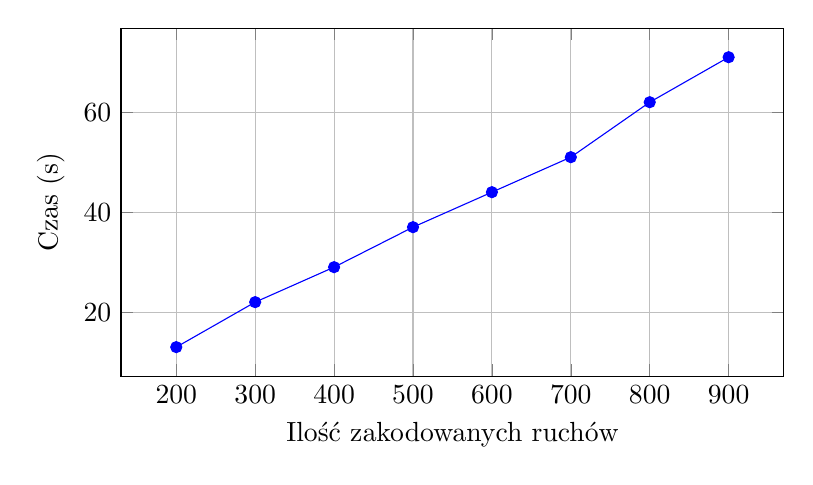
\begin{tikzpicture}
    \begin{axis}[
        xlabel={Ilość zakodowanych ruchów},
        ylabel={Czas (s)},
        grid=major,
        legend pos=north east,
        width=10cm,
        height=6cm
    ]
    \addplot[blue, mark=*] coordinates {
        (200, 13)
        (300, 22)
        (400, 29)
        (500, 37)
        (600, 44)
        (700, 51)
        (800, 62)
        (900, 71)
    };
    \end{axis}
    \end{tikzpicture}
    \caption{Czas wykonania metod concatenate po każdym zakodowaniu gry}
    \label{fig:concatenate_time}
\end{figure}
\section*{Biblioteka chess}
Biblioteka chess dostarcza zestaw podstawowych metod do pracy z szachami w pythonie. Umożliwia między innymi odczyt pliku pgn, stworzenie obiektu reprezentującego planszę szachową i wykonywanie na niej ruchów wraz z sprawdzaniem ich poprawności, a nawet umożliwia implementacje gotowego algorytmu jak stockfish. Działanie biblioteki opiera się na dwóch częściach: wizualizacyjnej oraz logicznej (todo: może zmienić).

\section*{Warstwa wizualizacyjna}
Warstwa wizualizacyjna jest bardzo prosta, gdyż przechowuje informacje o planszy w postaci ascii. Cała plansza jest zapisywana w postaci 8 linii oddzielonych znakiem "/". Każdy znak reprezentuje pierwszą literę angielskiej nazwy figury np: p od pawn, b od bishop itp. Dodatkowo w przypadku białych figur, jest to wielka litera, a w przypadku czarnych mała. Cyfry oznaczają ilość pustych pól. Na przykład: PPPP1PP oznacza cztery białe pionki, jedno puste pole oraz dwa białe pionki. Po zakodowanych polach planszy, występują dodatkowe informacje odzielonych spacją: kolor który wykonuje ruch, prawa do roszady, pola na których można wykonać bicie w przelocie, licznik półruchów oraz numer rundy. Konstruktor obiektu planszy przyjmuje między innymi jako argument \textit{fen}, czyli właśnie przedstawiony format. Daje to możliwość kopiowania oraz bardzo łatwego przesyłania dużej ilości informacji o planszy, co zostanie w dalszej części pracy wykorzystane.

\begin{lstlisting}[
    language=Python,
    caption=Przykład warstwy wizualizacyjnej,
    inputencoding=utf8,
    basicstyle=\ttfamily\footnotesize,
    backgroundcolor=\color{gray!10},
    frame=single,
    showspaces=false,
    showstringspaces=false,
    numbers=none
]
>>> board = chess.Board("r1bqkb1r/pppp1Qpp/2n2n2/4p3/2B1P3/8/PPPP1PPP/RNB1K1NR b KQkq - 0 4")
>>> print(board)
r . b q k b . r
p p p p . Q p p
. . n . . n . .
. . . . p . . .
. . B . P . . .
. . . . . . . .
P P P P . P P P
R N B . K . N R
\end{lstlisting}

\section*{Warstwa logiczna}
Warstwa logiczna jest znacznie bardziej rozbudowana. W postaci kilku liczb 64 bitowych przechowuje informacje o planszy. Każdy bit odpowiada jednemu polu na planszy. W ten sposób są zapisywane następujące informacje:

\begin{itemize}
    \item rodzaj figury
    \item kolor figury
    \item czy pole jest puste
    \item czy pole jest atakowane przez białe figury
    \item czy pole jest atakowane przez czarne figury
    \item czy figura jest z promocji
    \item czy figura ma prawo do roszady
\end{itemize}

\vspace{0.5cm}

\begin{lstlisting}[
    language=Python,
    caption=Przykładowy bitboard warstwy logicznej,
    inputencoding=utf8,
    basicstyle=\ttfamily\footnotesize,
    backgroundcolor=\color{gray!10},
    frame=single,
    showspaces=false,
    showstringspaces=false,
    numbers=none
]
>>> print(board)
r n b q k b n r
p p p p p p p p
. . . . . . . .
. . . . . . . .
. . . . . . . .
. . . . . . . .
P P P P P P P P
R N B Q K B N R

>>> BoardPlus.show_bitboard(board.rooks)
1 0 0 0 0 0 0 1
0 0 0 0 0 0 0 0
0 0 0 0 0 0 0 0
0 0 0 0 0 0 0 0
0 0 0 0 0 0 0 0
0 0 0 0 0 0 0 0
0 0 0 0 0 0 0 0
1 0 0 0 0 0 0 1
\end{lstlisting}


\section*{Klasa chessPlus}
Klasa chessPlus powstała jako rozszerzenie klasy Board z biblioteki chess. Naprawia ona kilka problemów związanych z zmianą perspektywy planszy, a także dodaje kilka bardzo ważnych metod enkodujących i dekodujących ruchy oraz plansze.

\section*{Zmiana perspektywy}
Zmiana perspektywy jest bardzo istotną częścią działania opisywanego algorytmu. Dzięki niej model nie musi uczyć się ruchów dla obu graczy, lecz jedynie dla białych figur. Zmiana perspektywy polega na zamianie kolorów oraz obróceniu planszy względem przekątnej. Czyli najpierw obracamy względem osi x, a następnie y. Biblioteka chess posiada w pełni działającą metodę \textit{apply\_mirror()}, która obraca planszę względem osi x, zmieniając jednocześnie kolory figur. Problem pojawia się przy obrocie względem osi y. Bilioteka zawiera generyczną metodę \textit{apply\_transform()} przyjmującą jako argument funkcję transformującą. W naszym przypadku jest to funkcja \textit{flip\_horizontal()}, która wykonuje operacje bitowe na opisujących plansze liczbach 64 bitowych. Mimo powyższych operacji, po wykonaniu obrotu nie działa poprawnie metoda \textit{push()}, która wykonuje ruch na planszy. Problemem są roszady...

\section*{Rozwiązanie problemu z roszadami}
Metoda \textit{push()} zaraz po wywołaniu sprawdza warunki roszady. Jeżeli nie są one spełnione to prawa do roszady zostają wyzerowane. Problem pojawia się w momencie kiedy plansza jest obrócona względem osi y. Autor biblioteki nie uwzględnił takiego obrotu i sztywno napisał warunki sprawdzające pozycje figur. Czego skutkiem są zerowane prawa do roszady. W celu naprawienia tego problemu, została stworzona metoda \textit{better\_clean\_castling\_rights()}, która uwzględnia obrót planszy.

\lstset{style=codeListingStyle}
\begin{lstlisting}[
    language=Python, 
    caption=poprawiony fragment metody clean castling rights,
    inputencoding=utf8
]
white_castling &= (chess.BB_A1 | chess.BB_H1)
black_castling &= (chess.BB_A8 | chess.BB_H8)

if not self.occupied_co[chess.WHITE] & self.kings & ~self.promoted & (chess.BB_D1 if self.changed_perspective else chess.BB_E1):
    white_castling = 0
if not self.occupied_co[chess.BLACK] & self.kings & ~self.promoted & (chess.BB_D8 if self.changed_perspective else chess.BB_E8):
    black_castling = 0

return white_castling | black_castling
\end{lstlisting}

W podobny sposób została naprawiona dalsza część metody \textit{push()} odpowiedzialna za roszady. W pierwszej kolejności została zdmodyfikowana metoda \textit{to\_chess960} tak aby uwzględniała transformacje planszy. Jest ona wywoływana na początku metody \textit{push()} i konwertuje ruch na standard chess960. Zamienia ona ruch w taki sposób, że przestawiając króla na pole obok wieży, zmienna \textit{move.to\_square} wskazywała na wieże. Takie obejście zostało zastosowane, gdyż biblioteka chess nie umożliwia formalnie postawienia swojej figury na zajętym polu przez swoje figury.

\begin{figure}[!h]
\centering
\includegraphics[width=0.8\textwidth]{images/board with castling.png}
\caption{Działanie metody to\_chess960}
\end{figure}

Po powyższych operacjach, metoda \textit{push()} usuwa figury i ustawia je na nowych pozycjach wraz z uwzględnieniem obrotu.

\section*{Dekodowanie planszy}
Dekodowanie planszy polega na stworzeniu 13 binarnych macierzy 8x8, gdzie każda z nich reprezentuje inny typ figury wraz z kolorem. Ostatnia z nich wskazuje na puste pola. Po zakodowaniu planszy, macieże są spłaszczane do jednego wektora o długości 832. 

\section*{Dekodowanie i enkodowanie ruchów}
Rodzai ruchów w szachach jest dokładnie 98. Jeżeli weźmiemy pod uwagę liczbę pól na planszy to jest ich dokładnie 6272. Są one zapisywane podobnie jak plansza, czyli w postaci trój wymiarowej macierzy 8x8x13. Gdzie pierwsze dwa wymiary reprezentują pole gdzie znajduje się figura, a trzeci wymiar reprezentuje indeks ruchu.

Ruchy pionka są najprostszymi ruchami, gdyż ograniczają się tylko do 4 ruchów: ruch do przodu i bicie na skos. Jako nieliczne są obliczane używając różnicy między docelowym, a obecnym polem. (\textit{move.from\_square - move.to\_square}). Zostały one zaprezentowane na poniższym rysunku:
\begin{figure}[!h]
\centering
\includegraphics[width=0.4\textwidth]{images/pawn_moves.png}
\caption{Indeksowanie ruchów pionka}
\end{figure}

Ruchy skoczka zostały zaimplementowane tak samo. Zostały one zaprezentowane na poniższym rysunku:

\begin{figure}[!h]
\centering
\includegraphics[width=0.4\textwidth]{images/knight_moves.png}
\caption{Indeksowanie ruchów skoczka}
\end{figure}

Indeksowanie ruchów gońca jest podzielone na lewą i prawą stronę. Dodatkowo jest uwzględniany wiersz na który chcemy wykonać ruch. Na przykład jeżeli chcemy wykonać ruch z pola E4 na C6 to jest to ruch w lewą stronę do wiersza 6, co jest reprezentowane przez indeks nr 25. Taki sposób działa niczym winda, gdzie wybieramy na jakie piętro chcemy wjechać. Sposób ten jest efektywny w porównaniu do obliczania różnicy pól, gdyż w najgorszym przypadku potrzebowalibyśmy aż 32 indeksów (4 strony po 8 wierszy), co jest 2 razy więcej niż opisywany sposób.
Indeksowanie ruchów wieży jest identyczne jak gońca, z tą różnicą że zamiast lewej i prawej strony, jest rozróznianie między ruchem pionowym i poziomym.
\begin{figure}[h]
\centering
\includegraphics[width=0.4\textwidth]{images/bishop_moves.png}
\hspace{1cm}
\includegraphics[width=0.4\textwidth]{images/rook_moves.png}
\caption{Indeksowanie ruchów gońca i wieży}
\end{figure}

Indeksowanie ruchów króla działa jak w przypadku pionków oraz skoczka. Natomiast hetman jest połączeniem ruchów gońca i wieży.

\begin{figure}[h]
\centering
\includegraphics[width=0.4\textwidth]{images/king_moves.png}
\hspace{1cm}
\includegraphics[width=0.4\textwidth]{images/queen_moves.png}
\caption{Indeksowanie ruchów króla i hetmana}
\end{figure}

\section*{Algorytm}
Zadaniem algorytmu w szachach jest znalezienie najlepszego ruchu w danej pozycji poprzez przewidywanie strategii przeciwnika. Słowo "strategia" jest kluczowe, gdyż odnosi się do planowania rozgrywki w przód, która ma na celu osiągnięcie celu w przyszłości, a nie w obecnym ruchu. Do tego celu idealnie nadają się algorytmy drzewiaste, które próbują przewidzieć przyszłość poprzez analizę kombinacji ruchów swoich jak i przeciwnika.

\section*{Drzewo minimax}
Drzewo minimax jest bardzo prostym jak i skutecznym algorytmem do przewidywania ruchów. Prostota polega na stworzeniu kombinacji wszystkich możliwych ruchów i wybranie ścieżki, która prowadzi do najlepszego wyniku. Nazwa wzięła się od tego, że algorytm gra sam ze sobą i wybiera ścieżkę minimalizując wynik przeciwnika równocześnie maksymalizując swój. 


% https://medium.com/@aidenrtracy/the-minimax-algorithm-f6e8e0a1eadb

\begin{figure}[!ht]
\centering
\includegraphics[width=0.4\textwidth]{images/minimax.jpg}
\caption{Drzewo minimax}
\end{figure}

\section*{Drzewo minimax w wersji alpha-beta}
Drzewo minimax w wersji alpha-beta jest zoptymalizowaną wersją algorytmu minimax. Eliminuje ona część gałęzi drzewa, dzięki czemu znacznie szybciej przeszukuje przestrzeń stanów. Jak sama nazwa wskazuje, wprowadza dodatkowo dwie zmienne alpha i beta. Alpha jest maksymalną wartością jaka może pojawić się w maksymalizującym węźle, a beta minimalną wartością jaka może pojawić się w minimalizującym węźle. Jeżeli podczas przeszukiwania drzewa wartość beta będzie mniejsza lub równa alpha to gałąź jest odcinana. Dzięki czemu unikamy niepotrzebnego przeszukiwania gałęzi drzewa, gdyż nie ma sensu sprawdzać ruchów, które nie moga bardziej zminimalizować, bądź zmaksymalizowac wyniku.

Złożoność czasowa minimax wynosi $O(b^d)$, gdzie $b$ to liczba możliwych ruchów w danym stanie, a $d$ to głębokość drzewa. W przypadku zastosowania alpha-beta, złożoność ta może zostać zredukowana do $O(b^{d/2})$ przy najlepszej kolejności ruchów. Możemy zauważyć, że w najlepszym przypadku jesteśmy w stanie stworzyć dwa razy głębsze drzewo.

\begin{figure}[!ht]
\centering
\includegraphics[width=0.6\textwidth]{images/alpha-beta.png}
\caption{Drzewo alpha-beta}
\end{figure}

\section*{Wady drzewa minimax}
Wyżej opisane drzewo minimax jest skuteczne do przewidywania ruchów w grach o małej przestrzeni stanów. W grach o większej złożoności takie jak szachy, zaczynają pojawiać się problemy. Ze względu na ograniczenia pamięciowe jak i czasowe, nie jest możliwe przeszukanie całego drzewa, nawet przy użyciu zoptymalizowanej wersji alpha-beta. Można ograniczyć głębokość drzewa, lecz w przypadku szachów jest to niemożliwe ze względu na brak metody oceniającej planszy w danym stanie. Rozwiązaniem tych problemów jest algorytm Monte Carlo Tree Search.

\section*{Drzewo monte carlo}
Algorytm Monte Carlo Tree Search jest heurystycznym algorytmem przeszukiwania zbioru stanów. Jego największą zaletą jest iteracyjność, dzięki czemu w zależności od dostępnej mocy obliczeniowej (czasu) możemy tworzyć dowolnie duże drzewo i po każdej iteracji jest w stanie zwrócić najlepszy ruch. Dodatkowo w podstawowej wersji nie wymaga skomplikowanej funkcji oceniającej dany stan. Działanie algorytmu opiera się na czterech etapach: selekcji, ekspansji, symulacji oraz wstecznej propagacji.

\begin{figure}[!ht]
\centering
\includegraphics[width=0.6\textwidth]{images/mcts_sections.png}
\caption{Etapy algorytmu Monte Carlo Tree Search}
\end{figure}

\section{Selekcja}
Etap selekcji, jak sama nazwa wskazuje wybiera najbardziej obiecujący liść do dalszego rozwoju drzewa. Liść jest rozumiany jako węzeł, który nie został jeszcze całkowicie rozwinięty, czyli nie posiada jeszcze wszystkich swoich dzieci.
Dany węzeł jest wybierany na podstawie maksymalizacji funkcji UCT:

\begin{equation}
\operatorname{UCT}(i) \,=\, \bar{x}_i \, + \, c\, \sqrt{\frac{\ln N}{n_i}}\,
\end{equation}

\noindent gdzie:
\begin{description}
  \item[$\bar{x}_i$] - średni wynik zwycięstw dla $i$-tego węzła
  \item[$n_i$] - liczba odwiedzeń $i$ - tego węzła
  \item[$N$] - liczba odwiedzeń węzła rodzica
  \item[$c$] - współczynnik eksploracji
\end{description}

\hspace{1cm}

Wzór ten składa się z sumy dwóch części. Pierwsza z nich $\bar{x}_i$ odpowiada za eksploatację, czyli wybór węzła, który jak dotąd osiągnął największy wynik. Druga część $c\, \sqrt{\frac{\ln N}{n_i}}$ skupia się na eksploracji, czyli wyborze węzła, który był rzadziej odwiedzany. Na poniżyszm wykresie możemy zauważyć, że część ta znacznie bardziej faworyzuje mniejszą liczbę odwiedzin $n_i$, ponadto użycie logarytmu naturalnego sprawia, że zmiana liczby odwiedzin węzła rodzica nie powoduje nagłych zmian w wartości eksploracji. Współczynnik $c$ we wzorze pozwala nam dostosować balans między eksploracją, a eksploatacją. Wyższa wartość $c$ faworyzuje eksplorację, natomiast niższa eksploatację.

\begin{figure}[!t]
\centering
\begin{tikzpicture}
\begin{axis} [
    xlabel={Liczba odwiedzin węzła $n_i$},
    ylabel={Wartość eksploracji},
    grid=major,
    width=10cm,
    height=6cm,
    domain=1:30,
    samples=200
]
\addplot[blue, thick] {sqrt(ln(50)/x)};
\legend{$\sqrt{\frac{\ln N}{n_i}}$}
\end{axis}
\end{tikzpicture}
\caption{Składnik eksploracji $\sqrt{\frac{\ln N}{n_i}}$ dla $N=100$}
\label{fig:uct-exploration}
\end{figure}

\section{Ekspansja}
Etap ekspansji ma za zadanie rozwijać drzewo poprzez dodanie jednego nowego węzła do wybranego liścia. Nowy węzeł jest wybierany losowo spośród wszystkich możliwych ruchów, które nie zostały jeszcze dodane do drzewa.

\section{Symulacja}
Etap symulacji polega na przeprowadzeniu symulacji rozgrywki \textbf{od} nowo dodanego węzła do końca gry w sposób losowy. W przypadku szachów oznacza to wykonywanie losowych ruchów aż do osiągnięcia stanu końcowego: mat, pat, remis.

\section{Wsteczna propagacja}
Etap wstecznej propagacji polega na propagowaniu wyniku symulacji w górę drzewa. Aktualizowane są wszystkie węzły od nowo dodanego węzła do korzenia. W każdym z tych węzłów zwiększana jest liczba odwiedzin, oraz sam wynik gry.


\section*{GUI}

Środowisko graficzne powstało w celu zobrazowania jak działa model w rzeczywistości. Zostało stworzone w języku Python z wykorzystaniem biblioteki PyGame. Działanie opiera się na zamianie obiektu board z biblioteki chess na plansze szachową z figurami, gdzie każda z nich jest w postaci zdjęcia z usuniętym tłem. Umożliwia również wykonywanie ruchów białymi figurami przez użytkownika. Interfejs graficzny dopuszcza i pokazuje tylko poprawne ruchy. W momencie gdy jest tura przeciwnika, wywoływany jest listener zwracający obiekt move. Taka struktura pozawala na bardzo łatwą implementację dowolnego algorytmu.

\begin{figure}[h]
\centering
\includegraphics[width=0.4\textwidth]{images/gui_czyste.png}
\hspace{1cm}
\includegraphics[width=0.4\textwidth]{images/gui_ruch.png}
\caption{intefejs graficzny}
\end{figure}

\lstset{style=codeListingStyle}
\begin{lstlisting}[
    language=Python, 
    caption=Przykładowe użycie gui,
    inputencoding=utf8
]
# obiekt board na ktorym dziala cala gra
board = BoardPlus() 

@torch.no_grad()
def algorithm():
    prob = chess_mctsnn.AMCTS(200, net).search(board)
    move_id = np.argmax(prob)
    move_mcts = board.decode_move(move_id)
    # zmiana perspektywy ruchu na czarne
    move_mcts = board.change_move_perspective(move_mcts)
    return move_mcts

game = chessGUI(board)
game.add_computer_algorithm_listener(algorithm)
game.run()
\end{lstlisting}
\section*{Źródła}
\begin{itemize}
    \item \url{https://www.chessprogramming.org/Forsyth-Edwards_Notation}
    \item \url{https://www.youtube.com/watch?v=UXW2yZndl7U}
    \item \url{https://www.youtube.com/watch?v=STjW3eH0Cik&t=2512s}
    \item \url{https://www.youtube.com/watch?v=wuSQpLinRB4&t=12193s}
    \item \url{https://vgarciasc.github.io/mcts-viz/}
    \item \url{https://python-chess.readthedocs.io}
    \item \url{https://medium.com/@aidenrtracy/the-minimax-algorithm-f6e8e0a1eadb}
    \item \url{https://gibberblot.github.io/rl-notes/single-agent/mcts.html}
    \item \url{https://www.geeksforgeeks.org/machine-learning/ml-monte-carlo-tree-search-mcts/}
\end{itemize}

\end{document}